% !TEX program = lualatex
% ECON 201, Worksheet 2: The Capitalist Takeoff. Compile with LuaLaTeX so the
% PDF is tagged (see syllabus/Econ201-Syllabus.tex for the same setup).
% Build from the course root:
%   latexmk -lualatex -cd worksheets/worksheet02.tex && latexmk -c -cd worksheets/worksheet02.tex
\DocumentMetadata{
  pdfstandard=UA-2,
  pdfversion=2.0,
  lang=en-US,
  tagging=on
}
\documentclass[11pt]{article}

\usepackage[letterpaper, margin=0.8in, top=0.6in, bottom=0.55in]{geometry}
\usepackage{fontspec}
\setmainfont{Fira Sans}
\usepackage{amsmath}
\usepackage{amssymb}
\usepackage{graphicx}
\usepackage{booktabs}
\usepackage{array}
% Questions are labelled by hand: under tagging=on, enumitem's enumerate
% did not step its counter, so every item printed the same label.
\newcounter{q}
\newcommand{\Q}[1]{\stepcounter{q}\par\needspace{5\baselineskip}\vspace{3pt}\noindent\hangindent=1.7em\hangafter=1
  \makebox[1.7em][l]{(\alph{q})}#1\par}
\usepackage{xcolor}
\usepackage{needspace}
\definecolor{accent}{HTML}{BF5700}
\usepackage{titlesec}
\titleformat{\section}{\large\bfseries\color{accent}}{}{0pt}{}
\titlespacing*{\section}{0pt}{6pt}{2pt}
\usepackage{hyperref}
\hypersetup{pdftitle={ECON 201 Worksheet: The Capitalist Takeoff}, pdfauthor={Div Bhagia}, hidelinks}
\pagestyle{empty}
\setlength{\parindent}{0pt}
\setlength{\parskip}{3pt}

% Ruled answer space: n lines. Plain TeX loop; pgffor's \foreach breaks the
% enumerate counter when used inside an item.
\newcount\answerlinecount
\newcommand{\answerlines}[1]{%
  \par\vspace{1pt}\answerlinecount=#1
  \loop\ifnum\answerlinecount>0
    \rule{\linewidth}{0.3pt}\par\vspace{5pt}%
    \advance\answerlinecount by -1
  \repeat
  \vspace{-5pt}}

\begin{document}

{\LARGE\bfseries\color{accent} Worksheet: The Capitalist Takeoff}\hfill{\large ECON 201}

\vspace{2pt}
Work with a neighbor. Write your answers in the spaces.

\needspace{7\baselineskip}\section{1. History's hockey stick}\setcounter{q}{0}

\begin{center}\vspace{-4pt}
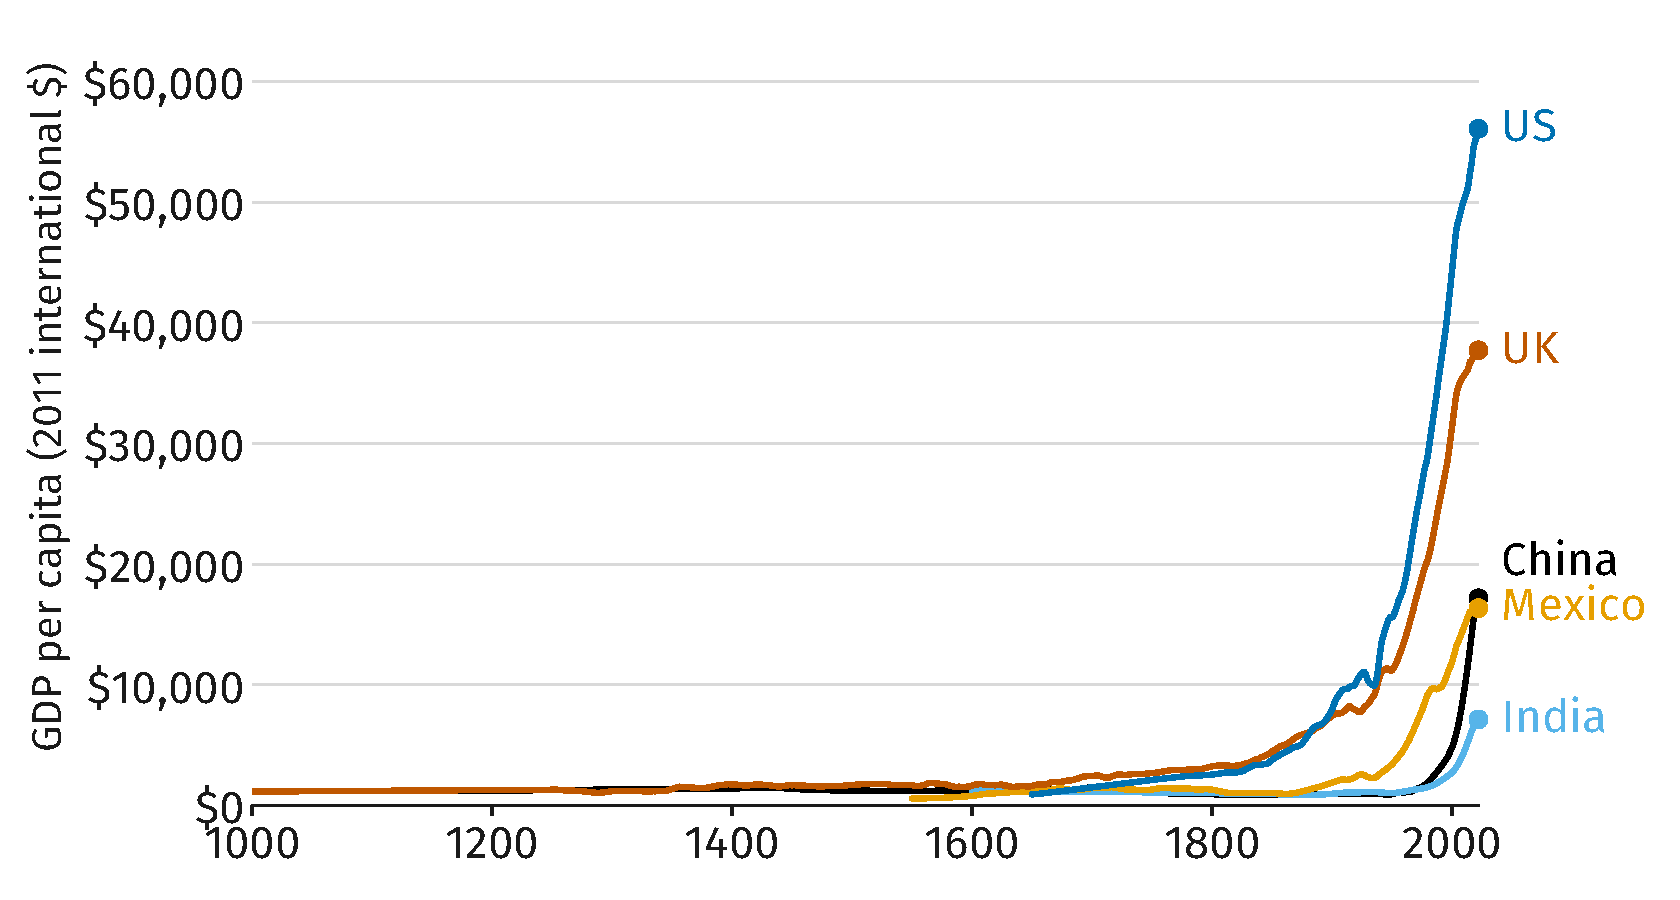
\includegraphics[width=0.8\textwidth, alt={GDP per capita in the UK, US, China, India, and Mexico from the year 1000 to 2022, in 2011 international dollars. Every line is nearly flat for centuries, then rises steeply after 1800. The US is highest at about 56,000 dollars, the UK near 38,000, then China, Mexico, and India below 20,000.}]{figures/hockey.pdf}
\vspace{-6pt}\end{center}

\textbf{When do living standards start to rise?} Estimate a year for each country from the chart. Think on your own for a minute, then compare with your neighbor.

\begin{center}
\renewcommand{\arraystretch}{1.35}
\begin{tabular}{@{}p{1.0in}p{1.8in}@{\hspace{0.6in}}p{1.0in}p{1.8in}@{}}
\toprule
Country & Rise begins around (year) & Country & Rise begins around (year) \\
\midrule
UK & \rule{1.4in}{0.3pt} & Mexico & \rule{1.4in}{0.3pt} \\
US & \rule{1.4in}{0.3pt} & China & \rule{1.4in}{0.3pt} \\
India & \rule{1.4in}{0.3pt} & & \\
\bottomrule
\end{tabular}
\end{center}

\needspace{7\baselineskip}\section{2. The three institutions of capitalism}\setcounter{q}{0}

Capitalism is an economic system built on three institutions: private property, markets, and firms.

\Q{For each example, check the institutions that are present.}

\begin{center}
\renewcommand{\arraystretch}{1.2}
\begin{tabular}{@{}p{3.4in}ccc@{}}
\toprule
 & Private property & Markets & Firms \\
\midrule
A family farm that grows food only for itself & $\square$ & $\square$ & $\square$ \\
A Saturday farmers' market & $\square$ & $\square$ & $\square$ \\
A state-owned steel mill in East Germany, 1970 & $\square$ & $\square$ & $\square$ \\
A ride-sharing company with 1,000 drivers & $\square$ & $\square$ & $\square$ \\
\bottomrule
\end{tabular}
\end{center}

\Q{Can a market work without private property? Why or why not? Can a firm exist without markets? Why or why not?}
\answerlines{3}

% ---------------------------------------------------------------------------
% Parked for later (practice problems or a future worksheet). These were
% drafted for this handout but cut so the in-class sheet holds two activities.
%
% \needspace{7\baselineskip}\section{2. Reading numbers off the chart}\setcounter{q}{0}
% 
% The UK line is at \$3,343 in 1800 and \$38,407 in 2022. In 2022, the US is at \$58,487 and India at \$7,766.
% \Q{How many times higher is UK GDP per capita in 2022 than in 1800?}
% \answerlines{1}
% \Q{By what percent did it change? Percent change $= \dfrac{\text{new} - \text{old}}{\text{old}} \times 100$.}
% \answerlines{1}
% \Q{In 2022, the average American is how many times richer than the average Indian?}
% \answerlines{1}
% 
% \newpage
% \section{3. Measuring prosperity}\setcounter{q}{0}
% 
% \Q{In one sentence: what is GDP per capita, and why do we divide by population?}
% \answerlines{1}
% \Q{A haircut costs 300 pesos in Mexico City and \$30 in Los Angeles. The exchange rate is 20 pesos per dollar. At the exchange rate, what does the Mexico City haircut cost in dollars? Why would converting Mexican incomes at the exchange rate understate what people there can buy?}
% \answerlines{2}
% 
% \needspace{7\baselineskip}\section{4. A natural experiment: the two Germanies}\setcounter{q}{0}
% 
% \begin{center}
% 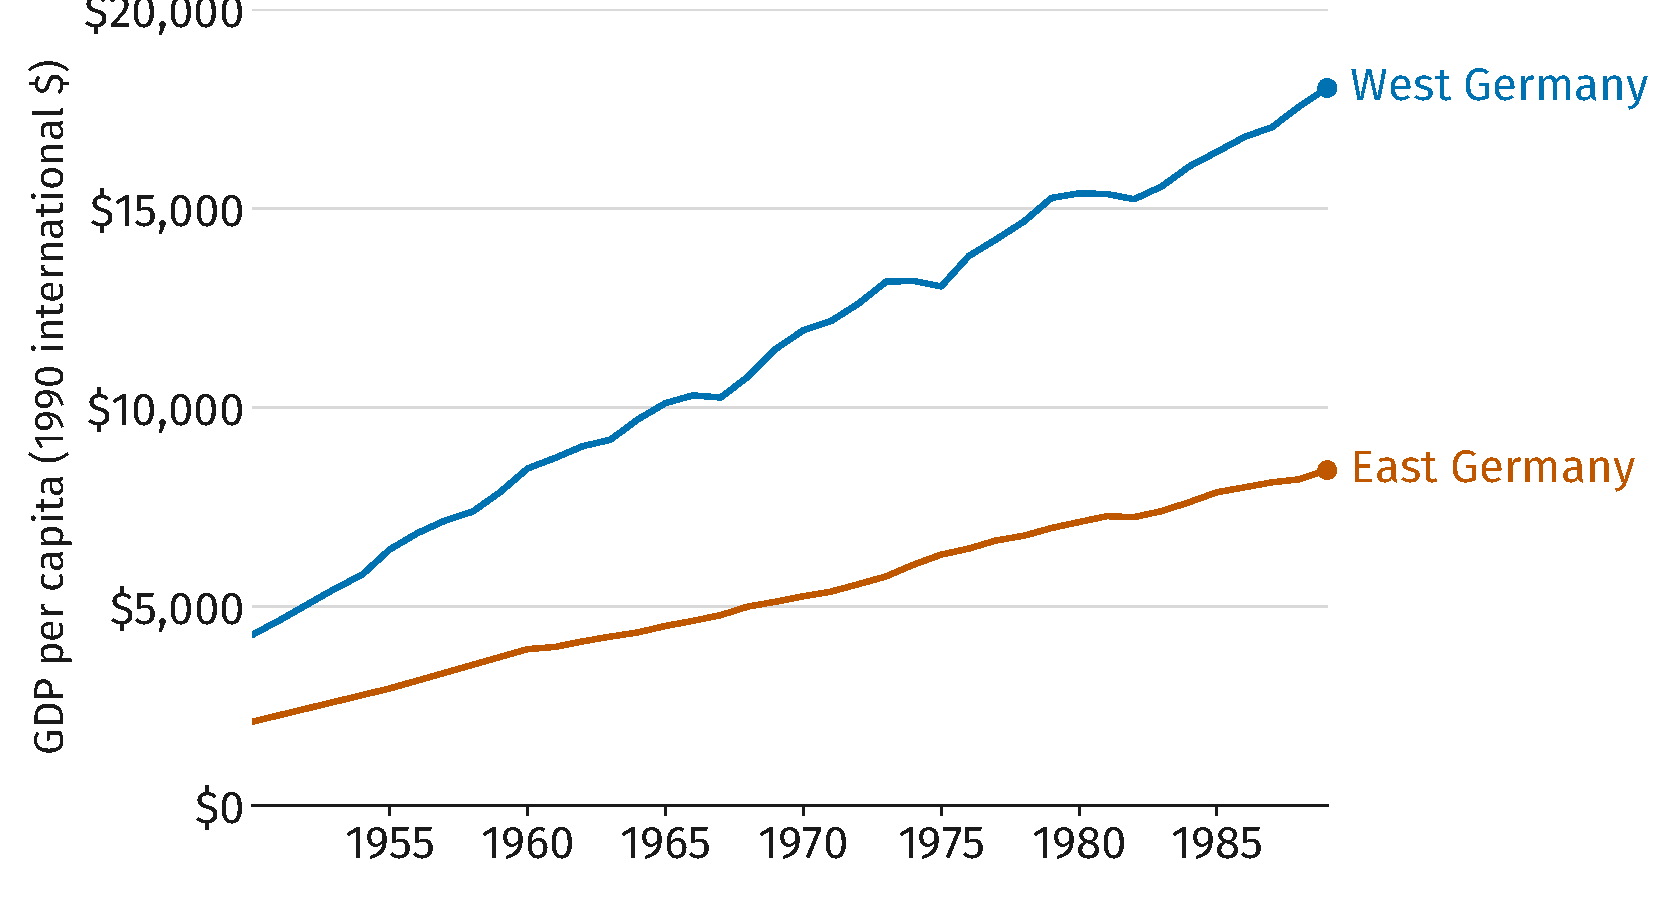
\includegraphics[width=0.46\linewidth, alt={GDP per capita in West Germany and East Germany from 1950 to 1989, in 1990 international dollars. West Germany rises from about 4,000 to 18,000 dollars; East Germany rises from about 2,000 to 8,000. The gap widens every decade.}]{figures/germanies.pdf}
% \vspace{-6pt}\end{center}
% 
% \Q{What was the same about the two Germanies in 1950? What was different after 1950?}
% \answerlines{2}
% \Q{What does the chart suggest caused the gap by 1989?}
% \answerlines{1}
% \Q{Why is this comparison more convincing than comparing, say, the US and India?}
% \answerlines{1}
% 
% \needspace{7\baselineskip}\section{5. The three institutions of capitalism}\setcounter{q}{0}
% 
% Capitalism is an economic system built on three institutions: private property, markets, and firms. For each example, check the institutions that are present.
% 
% \begin{center}
% \renewcommand{\arraystretch}{1.2}
% \begin{tabular}{@{}p{3.6in}ccc@{}}
% \toprule
%  & Private property & Markets & Firms \\
% \midrule
% A family farm that grows food only for itself & $\square$ & $\square$ & $\square$ \\
% A Saturday farmers' market & $\square$ & $\square$ & $\square$ \\
% A state-owned steel mill in East Germany, 1970 & $\square$ & $\square$ & $\square$ \\
% A ride-sharing company with 1,000 drivers & $\square$ & $\square$ & $\square$ \\
% \bottomrule
% \end{tabular}
% \end{center}
% 
% \needspace{7\baselineskip}\section{6. The other hockey stick}\setcounter{q}{0}
% 
% World carbon emissions have the same shape as the GDP chart: flat, then a steep rise after 1800. In one or two sentences, why do the two charts look alike?
% \answerlines{2}
% ---------------------------------------------------------------------------

\end{document}
